\chapter{Rezultate experimentale}
\thispagestyle{pagestyle}

Un prim experiment efectuat a fost expunerea ansamblului de alarmă la gaze și fum folosind o brichetă. În Figura \ref{fig:chart_gaze} se pot observa fluctuațiile valorilor pentru fum și gaz în intervalul 3:55 - 3:57, timp în care a fost efectuat experimentul. Folosind bricheta, am umplut camera din machetă unde se află senzorul MQ2, răspunsul sistemului fiind cel aștept: atât aplicația mobile, cât și interfața de pe platforma Blynk au arătat aceleași valori crescute, iar alarma a fost declanșată timp de trei secunde pe perioada fiecărei detecții.

\begin{figure}[H]
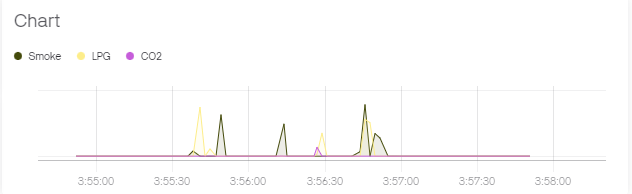
\includegraphics[width=0.8\linewidth]{bachelors_ro/images/chart_gaze.png}
\caption{Nivelul de gaze și fum detectat în urma experimentului}
\label{fig:chart_gaze}
\end{figure}

Un alt experiment efectuat a fost deconectarea sursei ce alimentează ventilatorul și becul pentru a lăsa senzorul să ajungă la temperatura ambientală. Am așteptat până temperatura s-a stabilizat la aproximativ 21 de grade, apoi am reconectat sursa și am setat temperatura dorită la 27 de grade.

\begin{figure}[H]
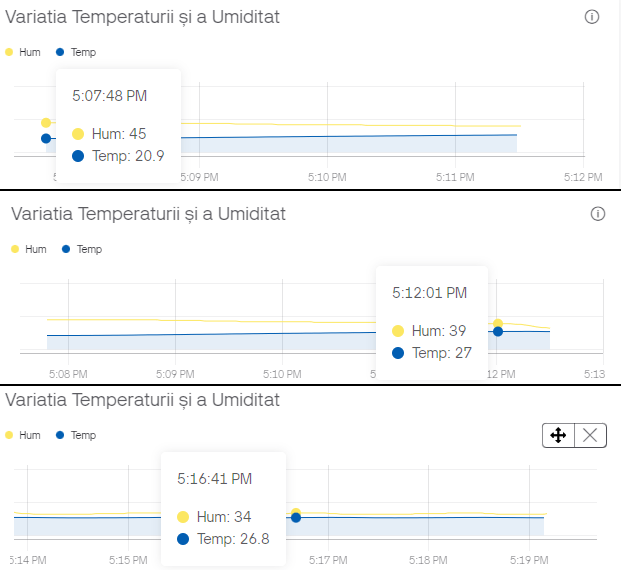
\includegraphics[width=0.5\linewidth]{bachelors_ro/images/combined_chart.png}
\caption{Grafice cu valorile temperaturii în timpul experimentului}
\label{fig:combined_chart}
\end{figure}

Plecând de la 21 de grade Celsius se poate observa în Figura \ref{fig:combined_chart} că termostatul a ajuns la temperatura setată de 27 de grade Celsius în aproximativ 4 minute (intervalul de timp 5:07:48 în primul grafic - 5:12:01 în al doilea grafic). În cel de-al treilea grafic se poate observa stabilitatea sistemului existând variații minore ale temperaturii de +/- 0.5 grade Celsius pe un interval de 5 minute. Concluzionând, ansamblul de stabilizare a temperaturii funcționează corect oferind valori aproape constante, dar și eficient reușind să încălzească 6 grade în doar 4 minute.

\section{Realizarea machetei}

Macheta ce găzduiește sistemul implementat este reprezentată de o casă făcută din plăci de lemn. În Figura \ref{fig:casa_init} se poate observa structura de la care s-a pornit, aceasta fiind un simplu paralelipiped gol. 

\begin{figure}[H]
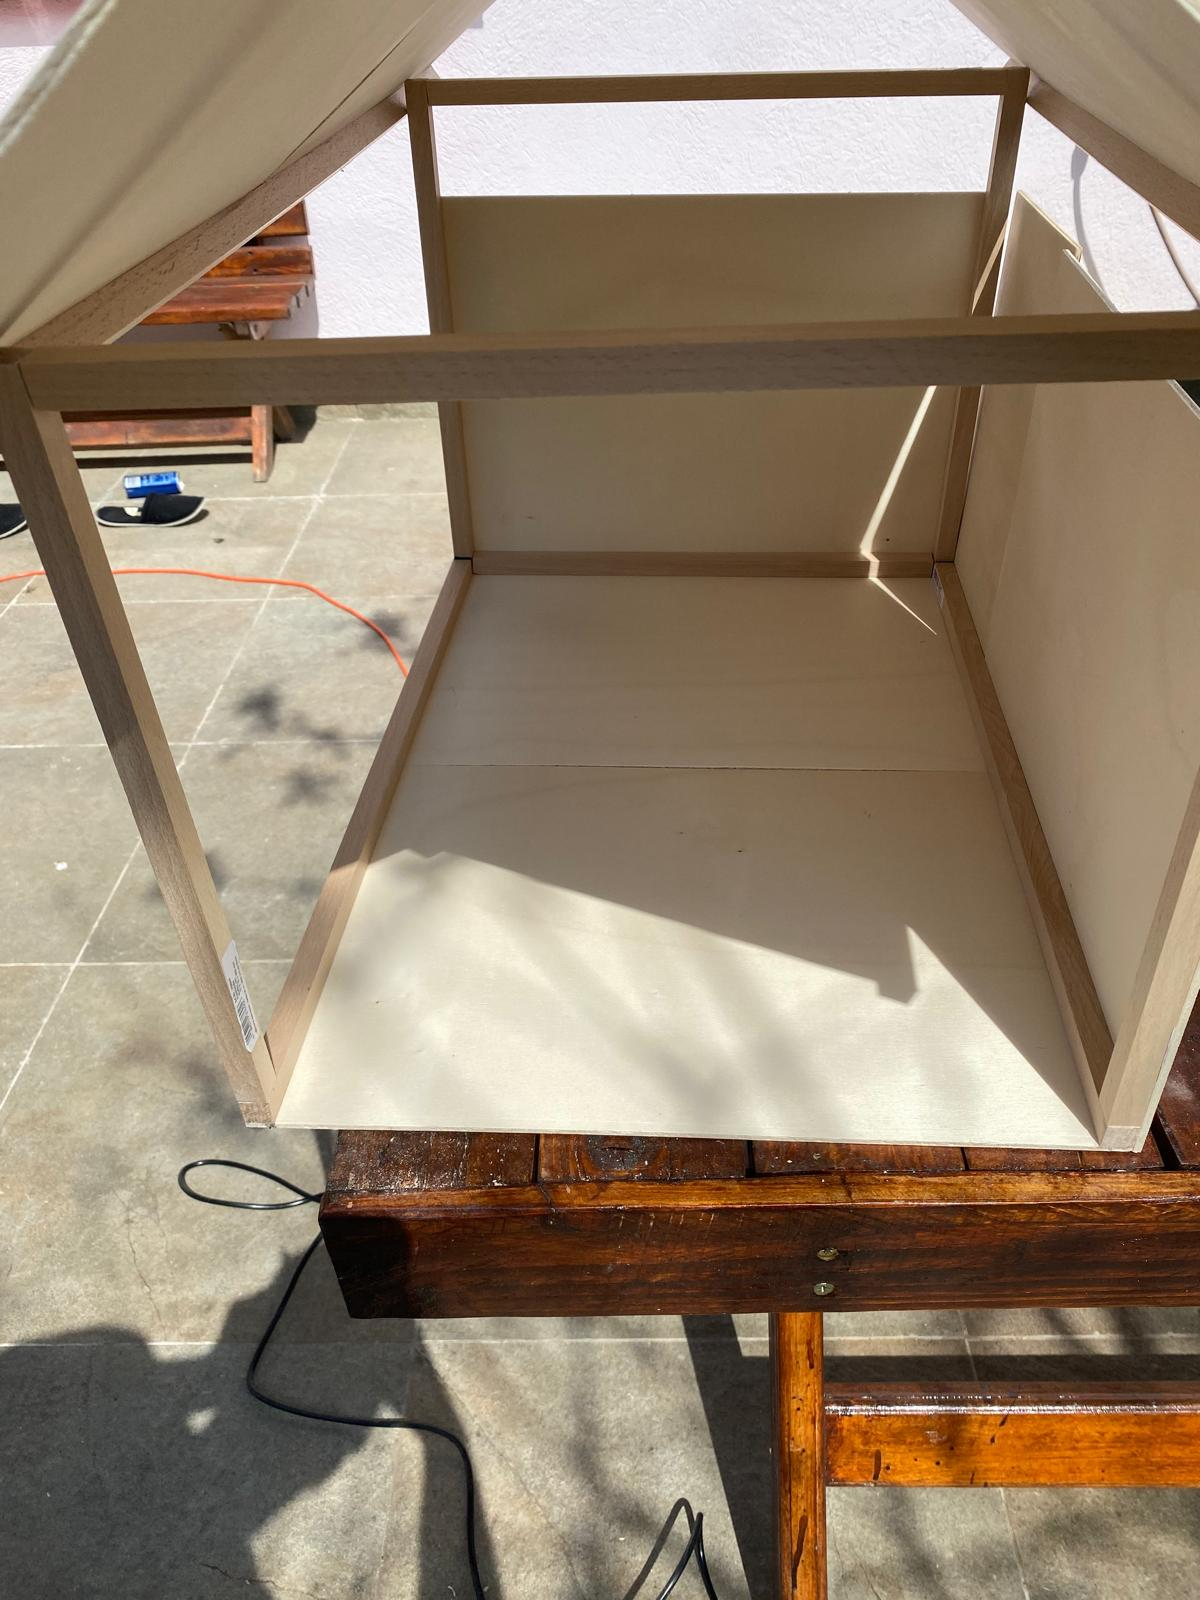
\includegraphics[width=0.3\textwidth, height=0.4\textwidth]{bachelors_ro/images/casa_init.jpg}
\caption{Macheta în stare incipientă}
\label{fig:casa_init}
\end{figure}

În continuare, am decis să construiesc două etaje, la primul etaj să fie folosite 3 camere individuale, una pentru alarma de gaz, una pentru senzorul de mișcare și led-ul controlat aferent și una pentru ușa automată. Astfel, am adăugat pereții necesari și am adăugat o podea pentru al doilea etaj ce reprezintă în același timp și tavanul primului etaj.

În Figura\ref{fig:schema_casa} se poate observa schema casei. Dimensiunile acesteia sunt: L 60 cm x l 42 cm x H 38 cm. Fiecare componentă a fost așezată într-una dintre camere: 1 - senzorul pir și led-ul aferent acestuia, 2 - ansamblul de alarmă, led-ul aferent modului cu fotorezistor și  senzorul BMP280, 3 - ansamblul de stabilizare a temperaturii, 4 - ansamblul de deschidere automată a ușii, 5 - modulul cu fotorezistor.

\begin{figure}[H]
    \centering
    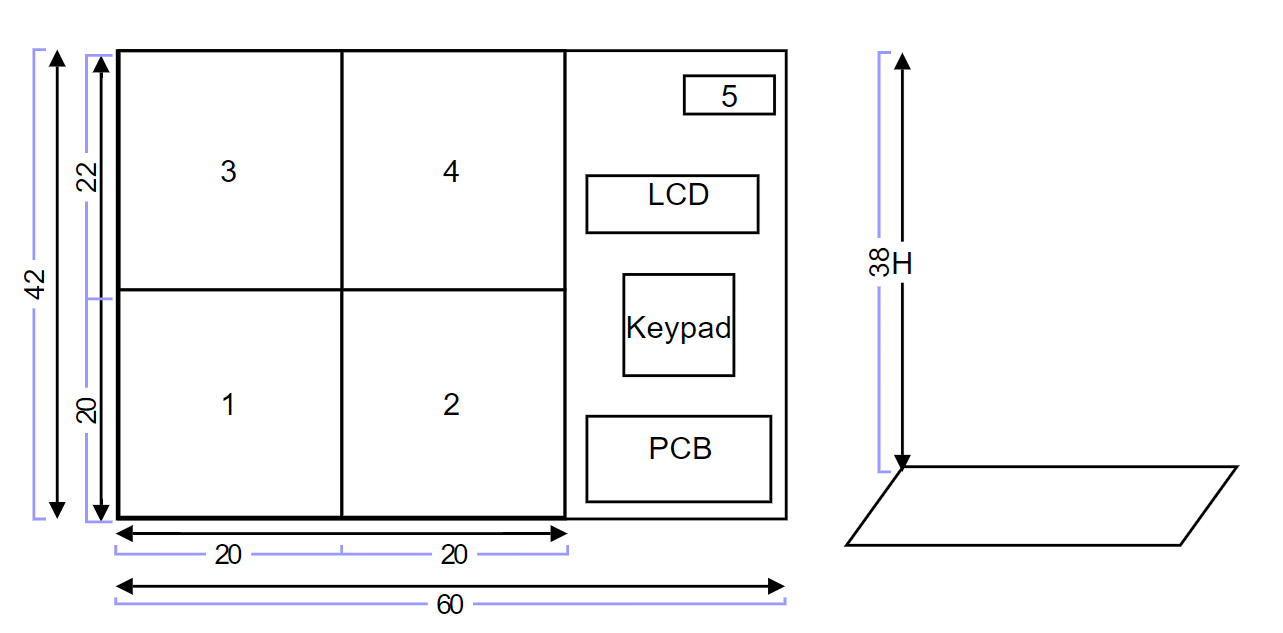
\includegraphics[width=0.8\linewidth]{bachelors_ro/images/schema_casa.png}
    \caption{Schema casei}
    \label{fig:schema_casa}
\end{figure}

Următorul pas după delimitarea arhitecturii a fost decuparea placajului pentru a permite trecerea cablurilor și, unde este cazul, încastrarea componentelor. Ultimul pas a fost să izolez zona ce conține ansamblul de stabilizare a temperaturii în plexiglas. 

În Figurile \ref{fig:casa_din_fata} \ref{fig:casa_de_sus} și \ref{fig:casa_din_lateral} se poate observa rezultatul final al realizării machetei.

\begin{figure}[H]
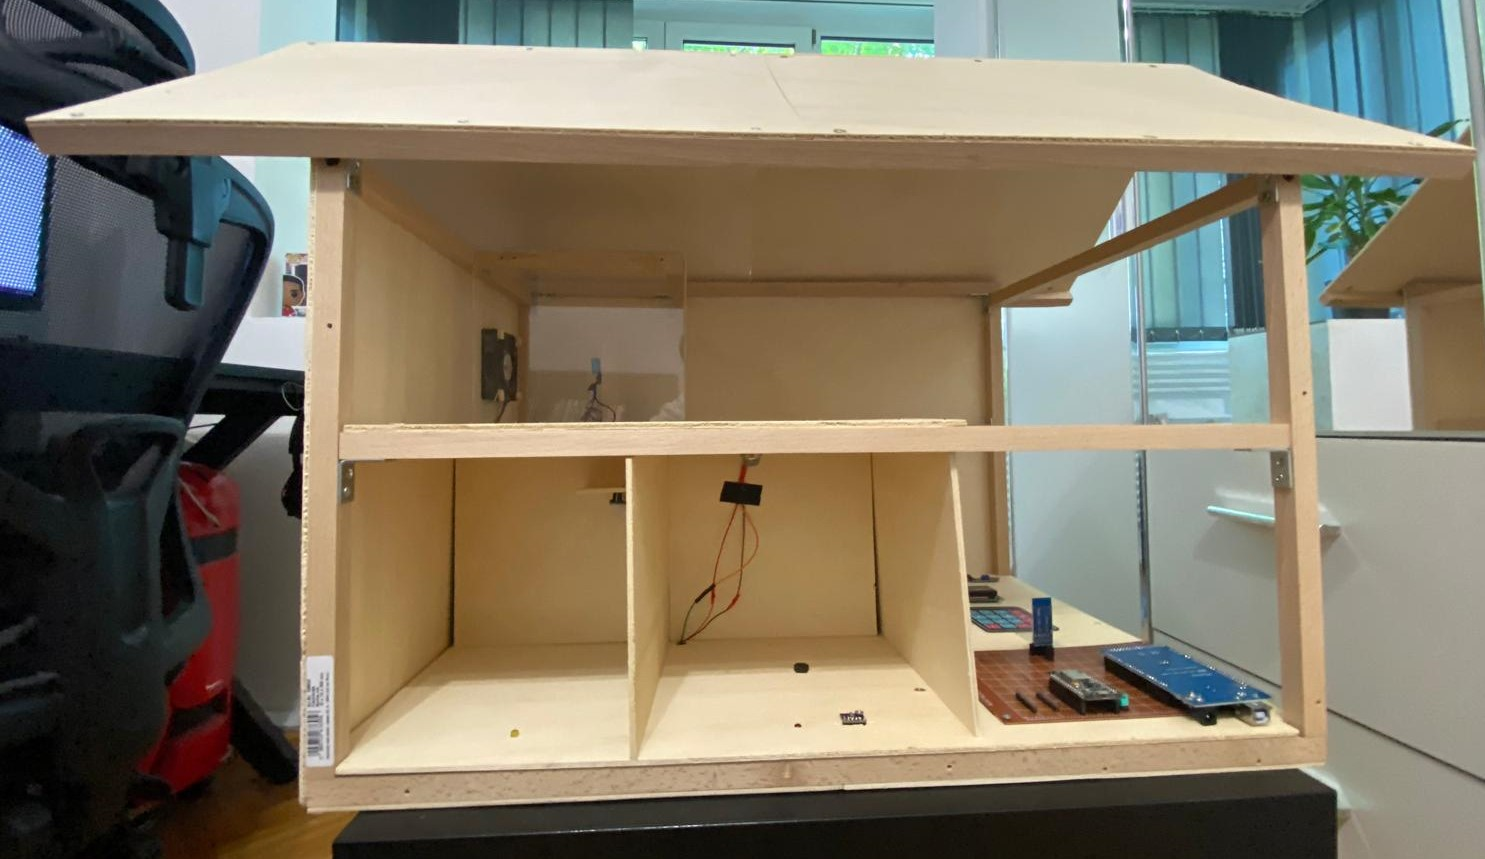
\includegraphics[width=0.6\linewidth]{bachelors_ro/images/casa_din_fata.jpg}
\caption{Macheta văzută din față}
\label{fig:casa_din_fata}
\end{figure}

\begin{figure}[H]
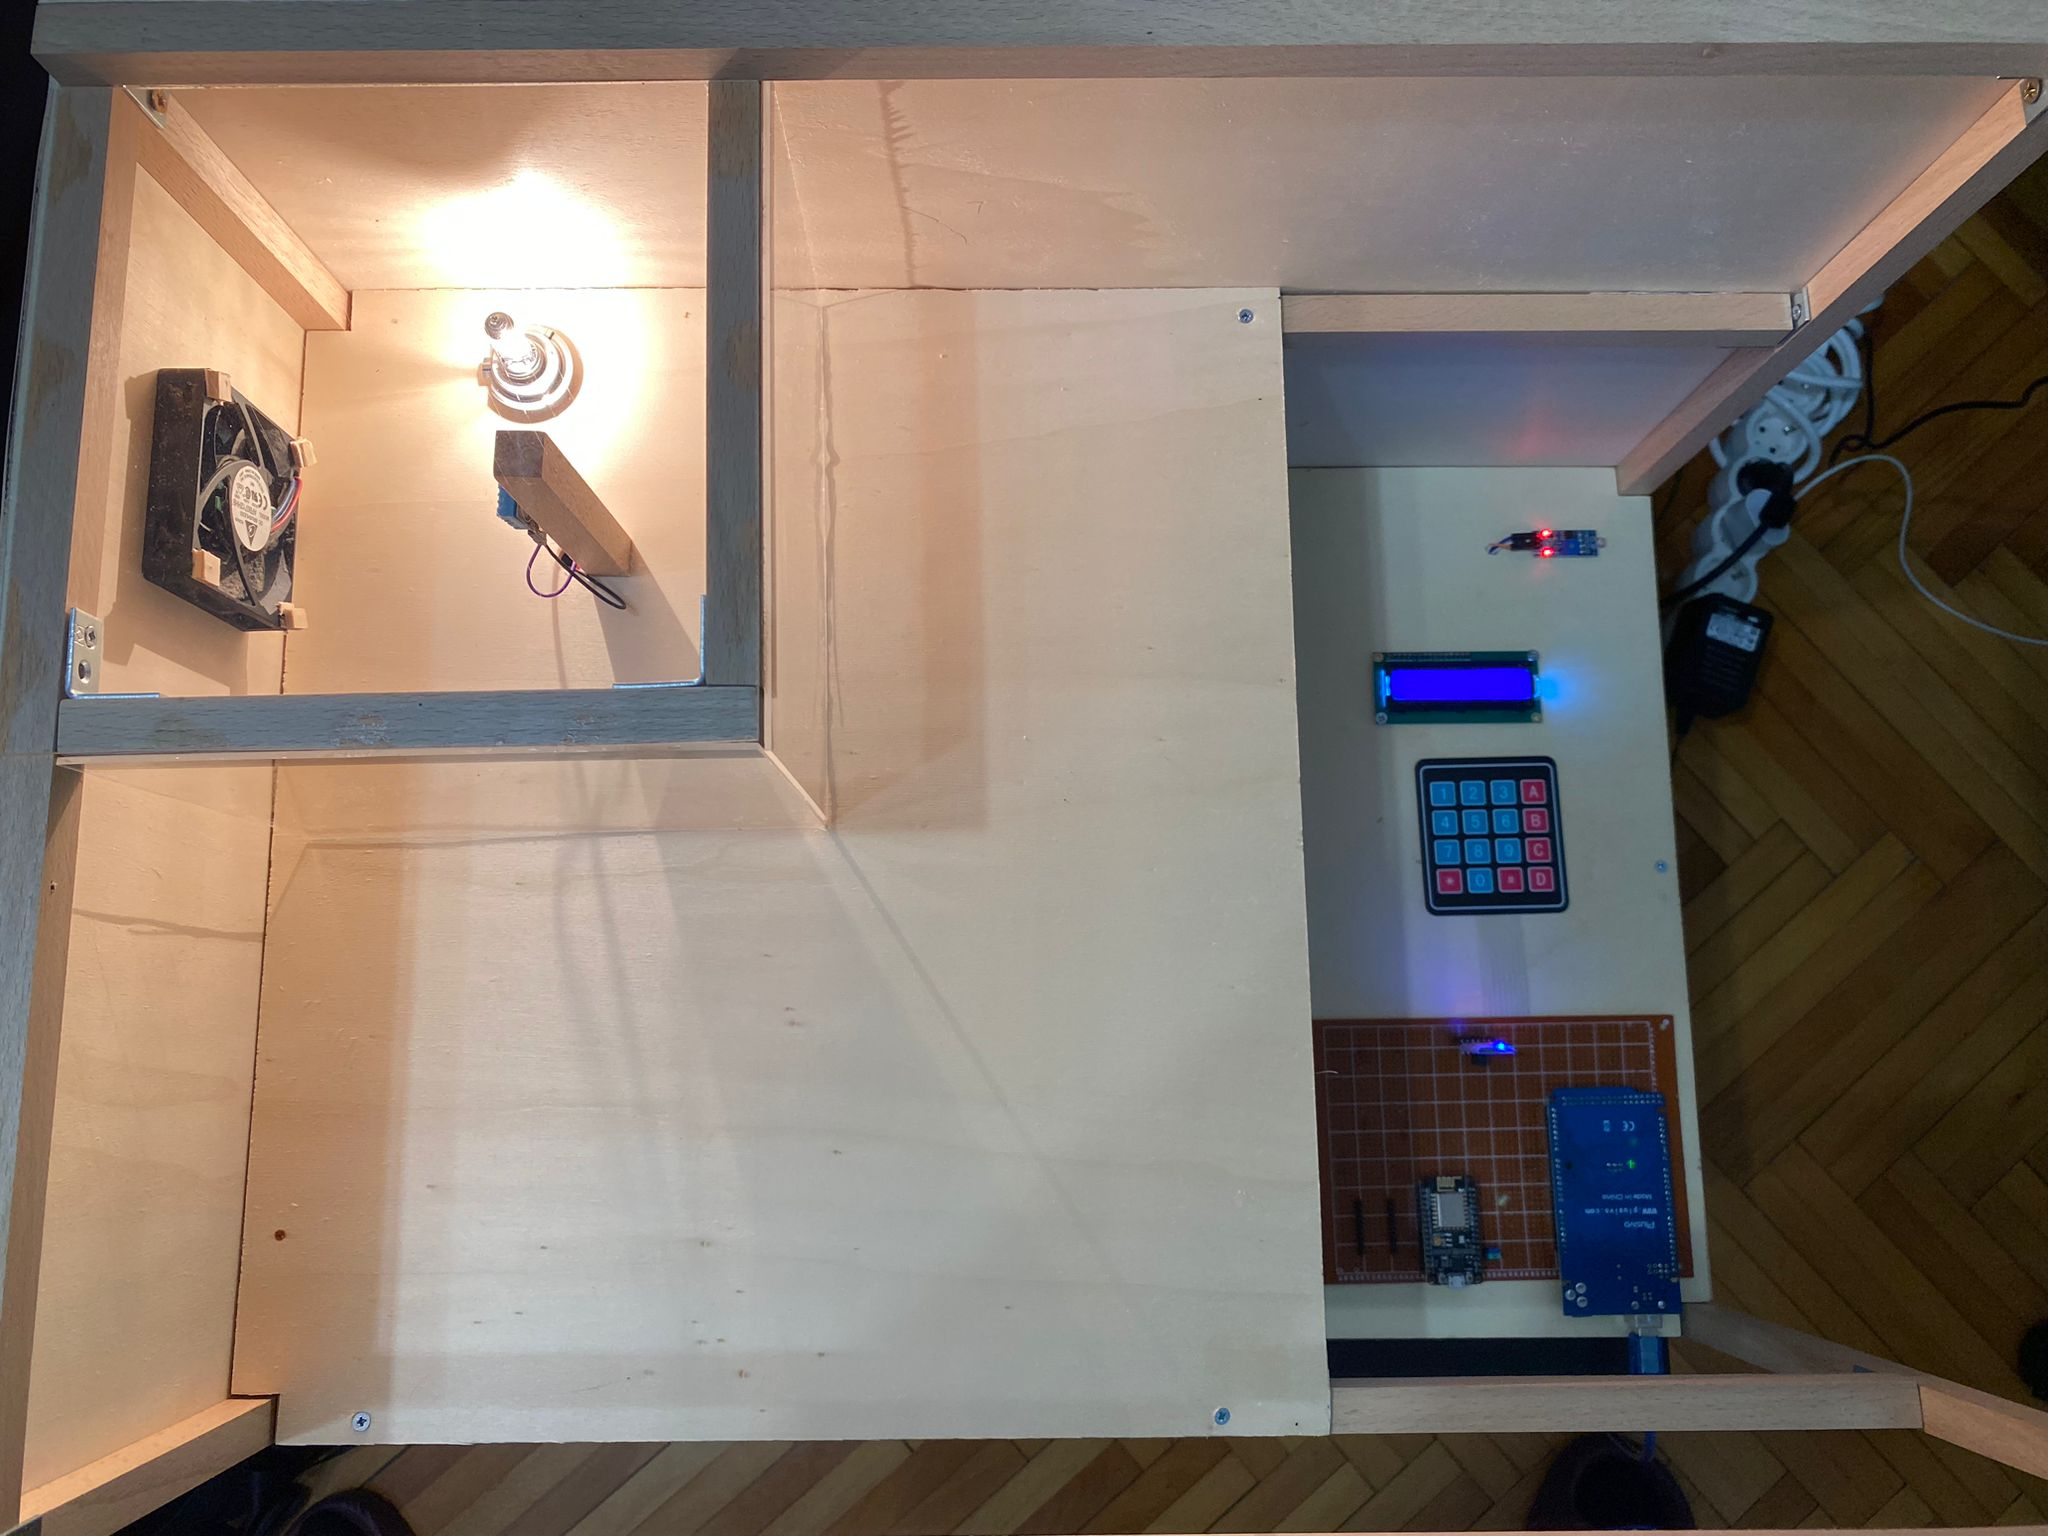
\includegraphics[width=0.6\linewidth]{bachelors_ro/images/casa_de_sus.jpg}
\caption{Macheta văzută de sus}
\label{fig:casa_de_sus}
\end{figure}

\begin{figure}[H]
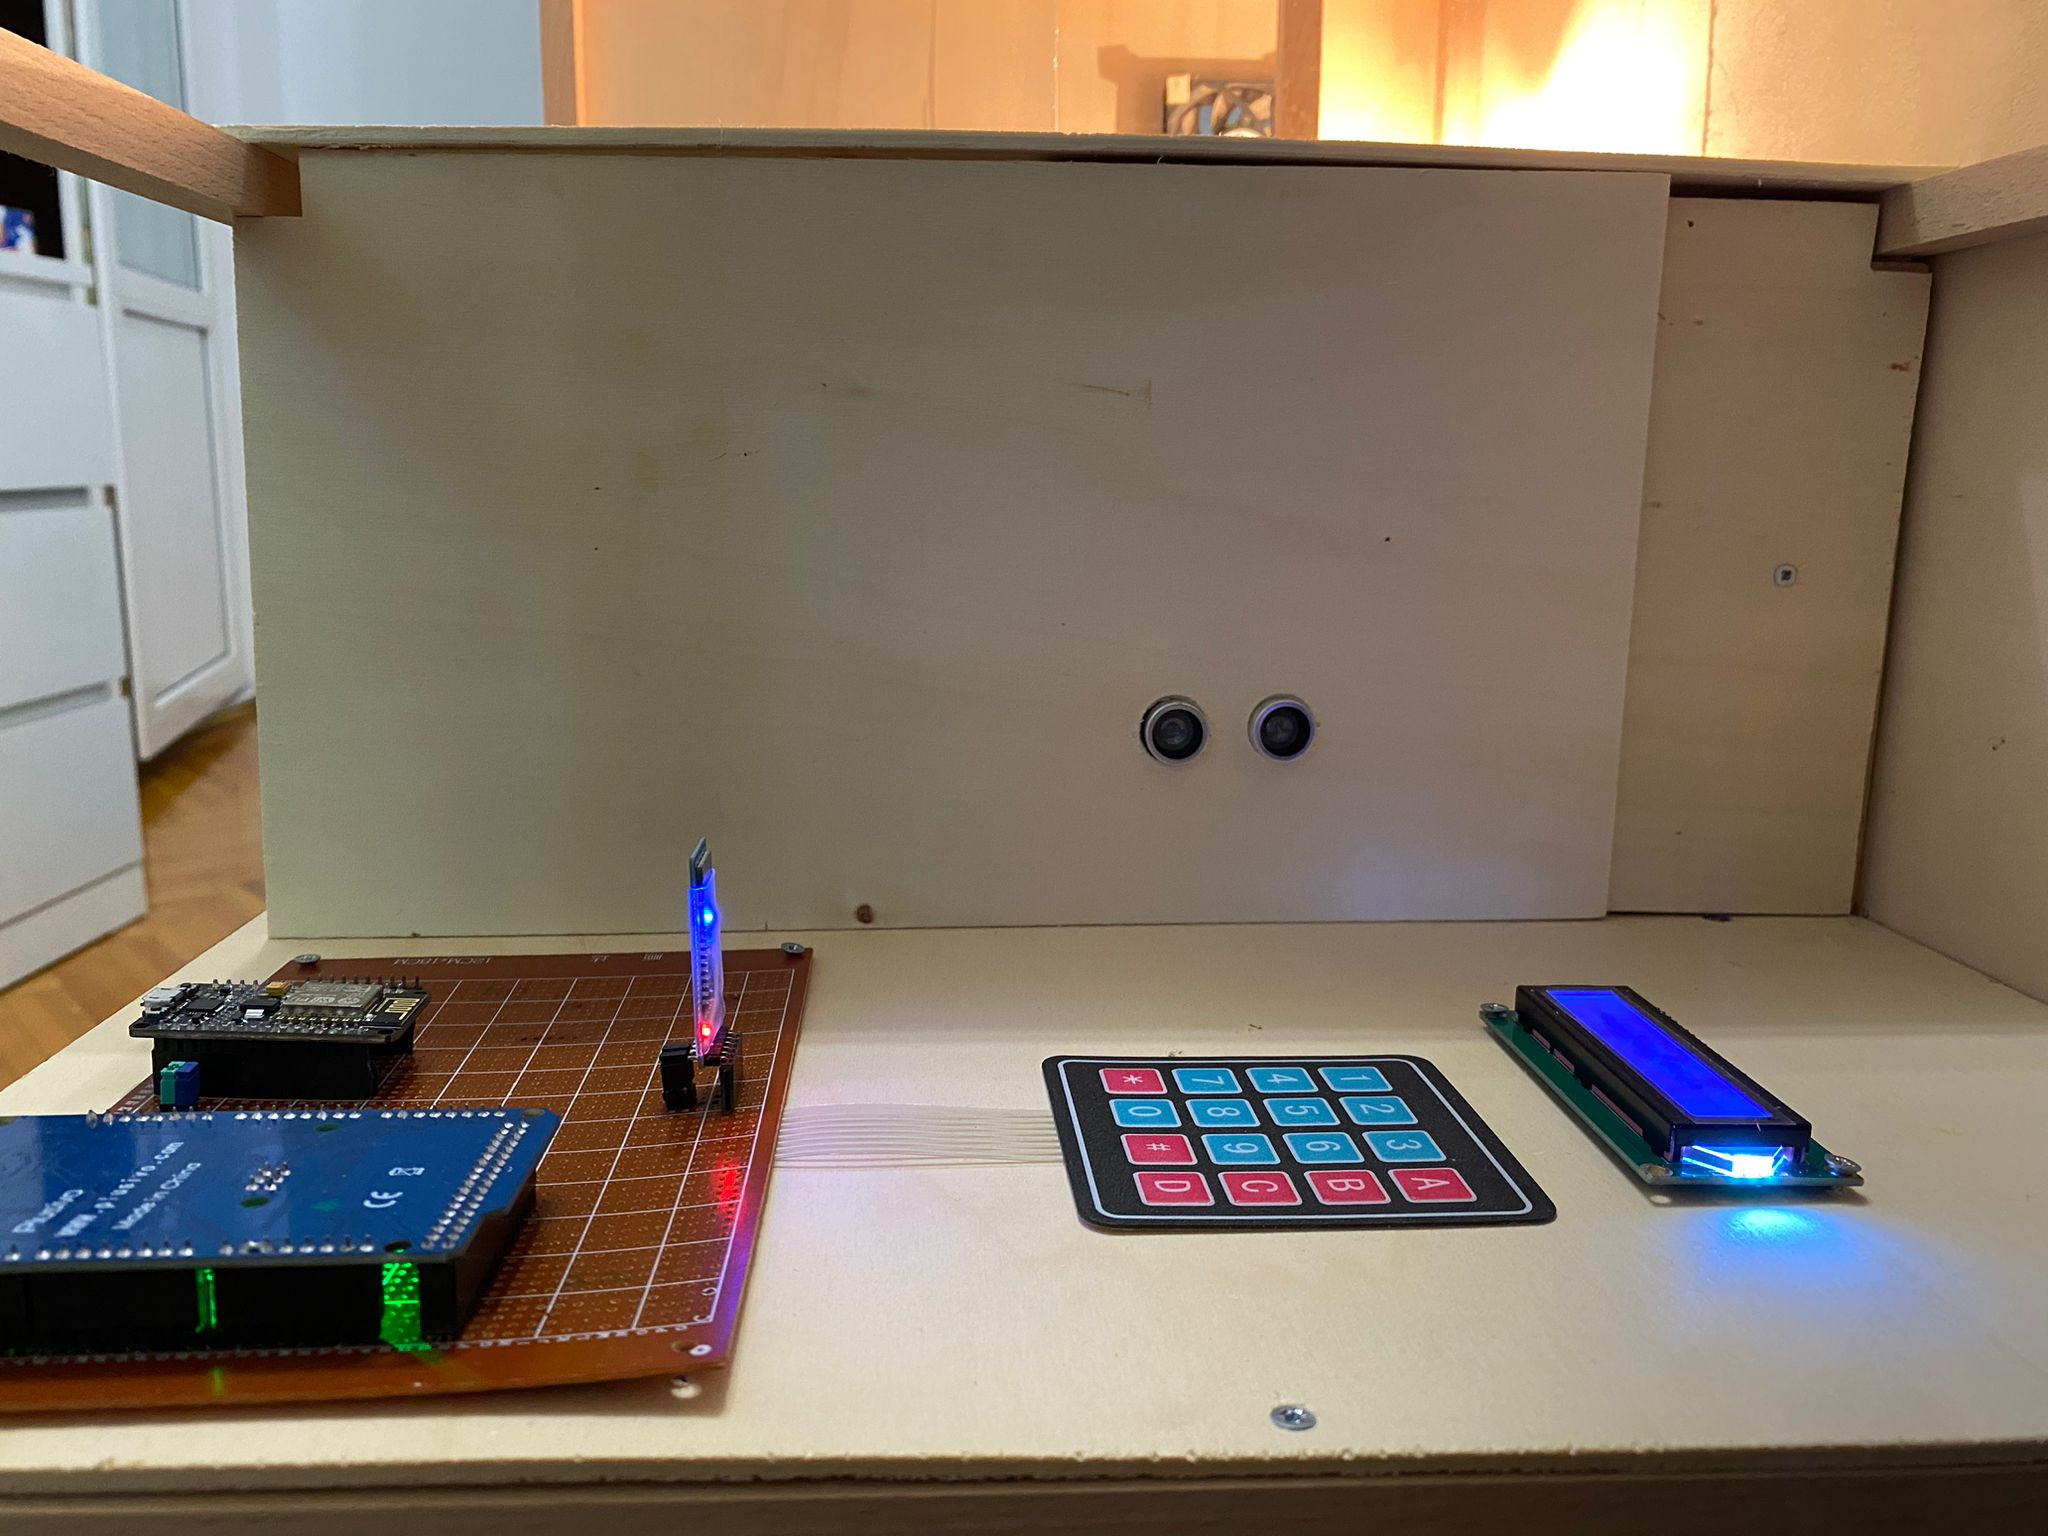
\includegraphics[width=0.6\linewidth]{bachelors_ro/images/casa_din_lateral.jpg}
\caption{Macheta văzută din lateral}
\label{fig:casa_din_lateral}
\end{figure}

Cablajul a fost realizat inițial la nivel de breadboard (Figura \ref{fig:cablaj_breadboard}. Apoi am realizat că această variantă nu este practică deoarece cablurile se pot deconecta oricând. Astfel am decis să folosesc o placă PCB și să cositoresc toate firele de aceasta creând practic un nucleu al sistemului.

\begin{figure}[H]
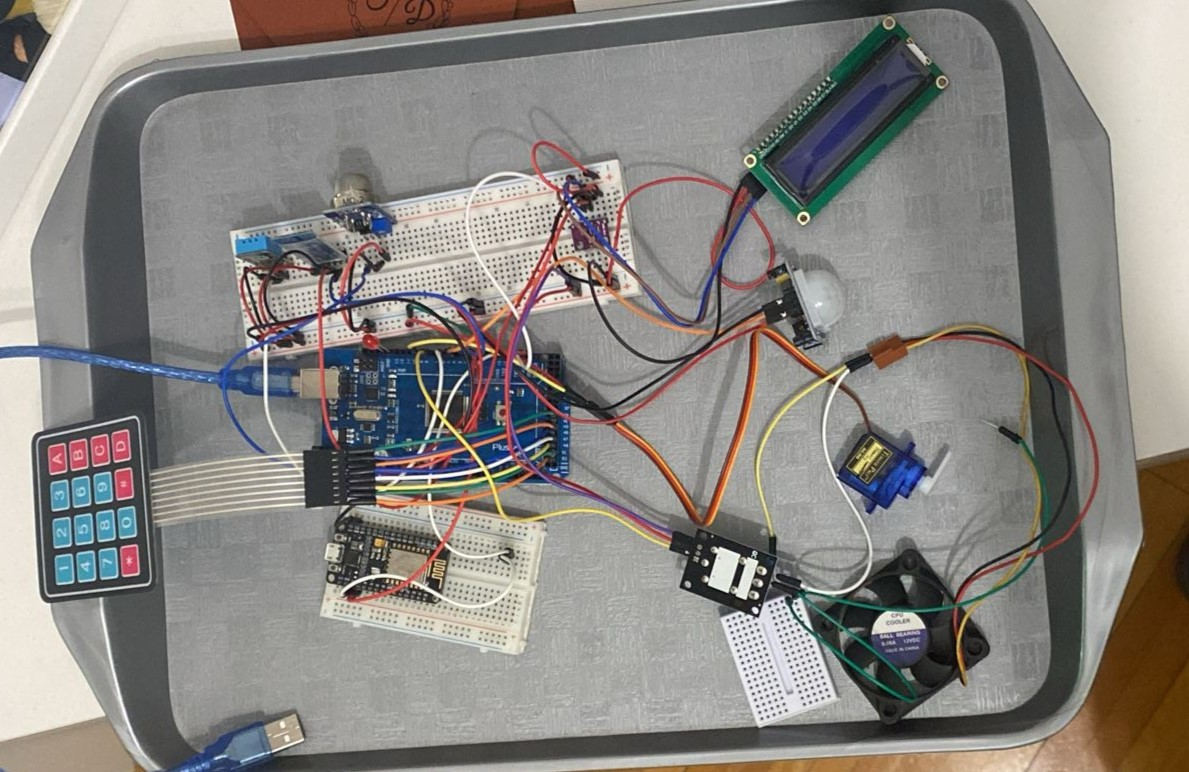
\includegraphics[width=0.6\linewidth]{bachelors_ro/images/cablaj_breadboard.jpg}
\caption{Cablaj la nivel de breadboard}
\label{fig:cablaj_breadboard}
\end{figure}

În Figura \ref{fig:cablaj_pcb} se poate observa cablajul montan pe placa PCB. Această placă este încastrată în podeaua machetei. În Figura\ref{fig:pcb_fata} este prezentată placa PCB pe care s-a montat placa de dezvoltare Arduino Mega, modulul NodeMCU și modulul Bluetooth. Macheta dispune de o podea dublă pentru un management al cablurilor facil, acest fapt este prezentat în Figura \ref{fig:podea_dubla}.

\begin{figure}[H]
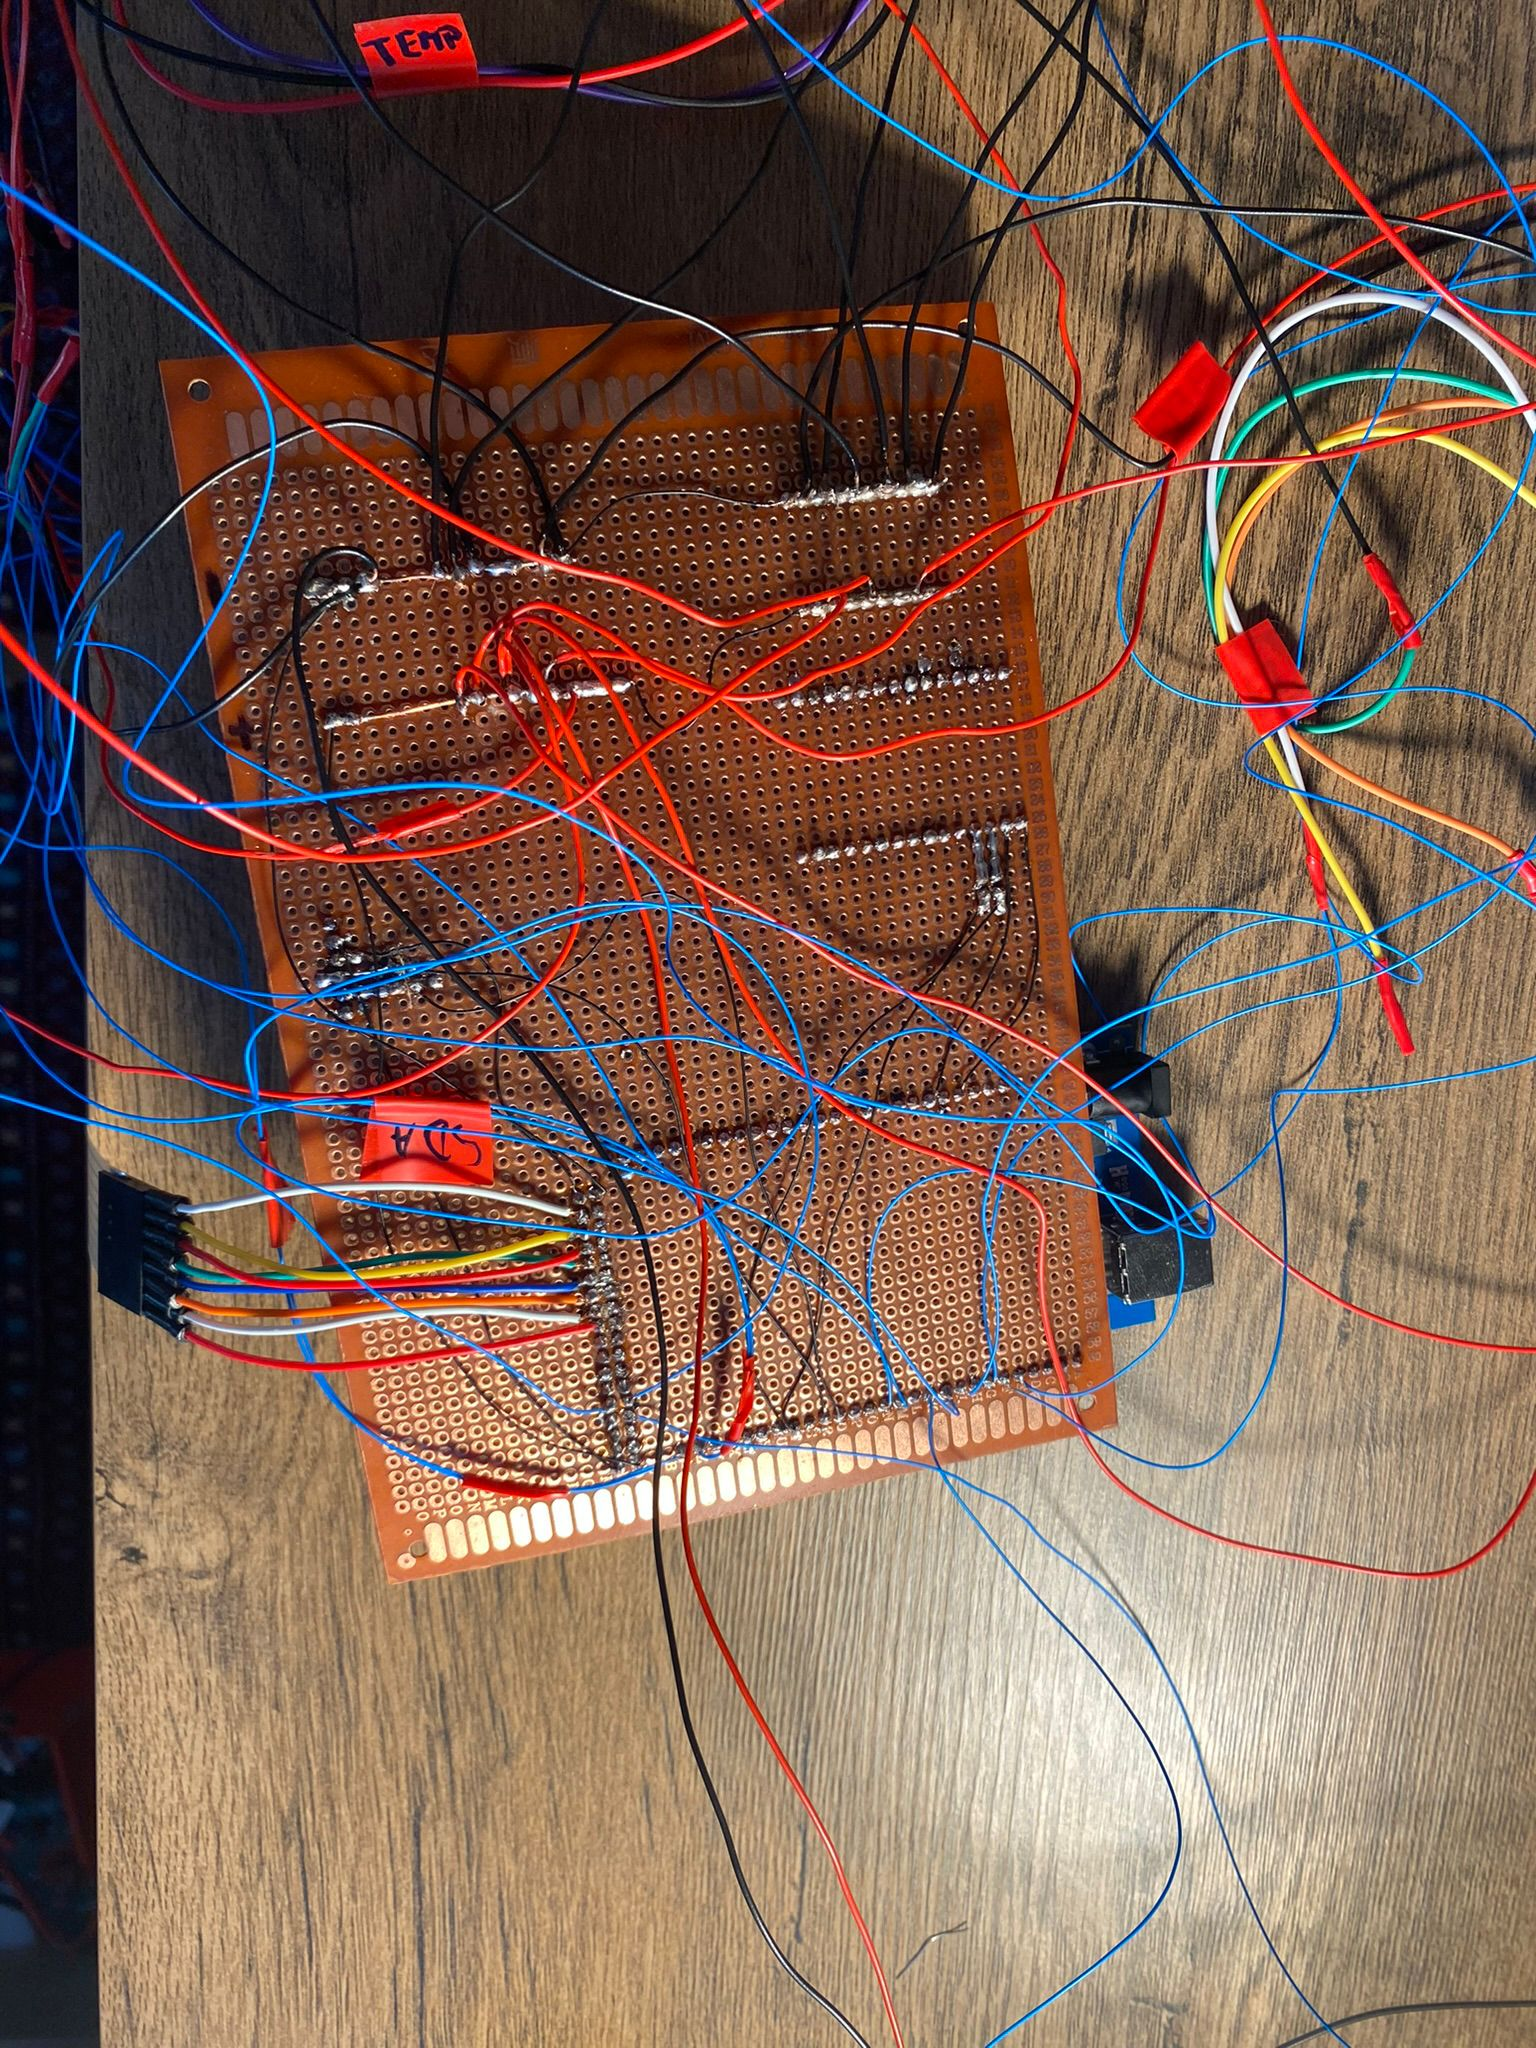
\includegraphics[angle=90,width=0.7\linewidth]{bachelors_ro/images/cablaj_pcb.jpg}
\caption{Cablaj pe placa PCB}
\label{fig:cablaj_pcb}
\end{figure}

\begin{figure}
    \centering
    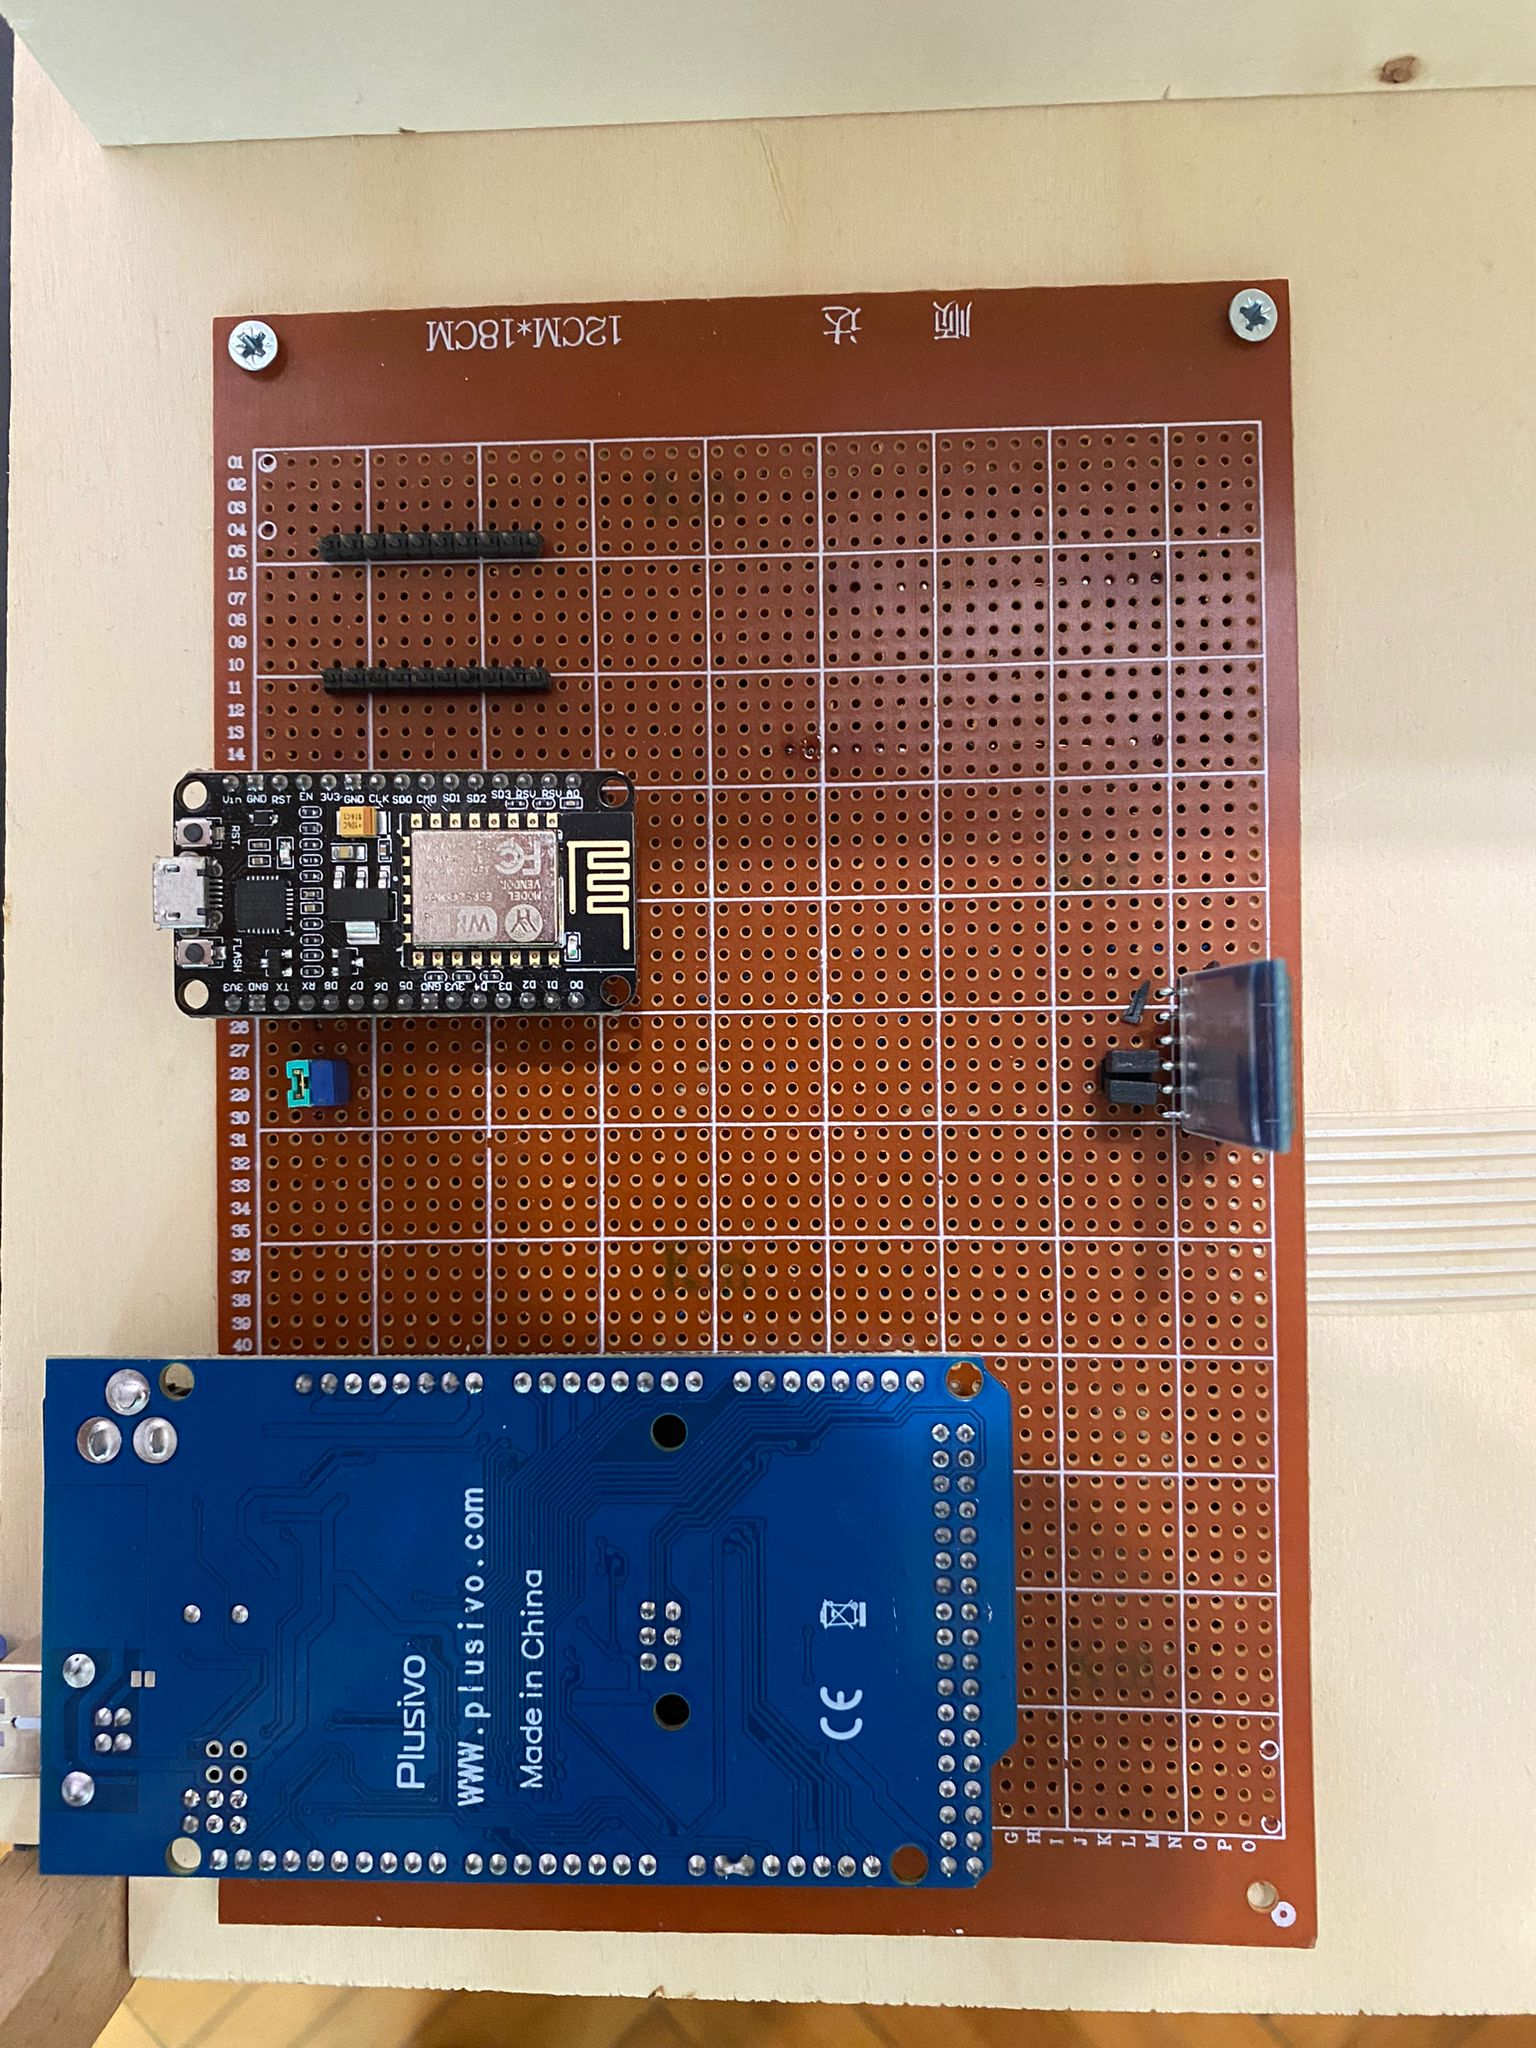
\includegraphics[angle=90,width=0.7\linewidth]{bachelors_ro/images/pcb_fata.jpg}
    \caption{Placa PCB văzută de sus}
    \label{fig:pcb_fata}
\end{figure}

\begin{figure}[H]
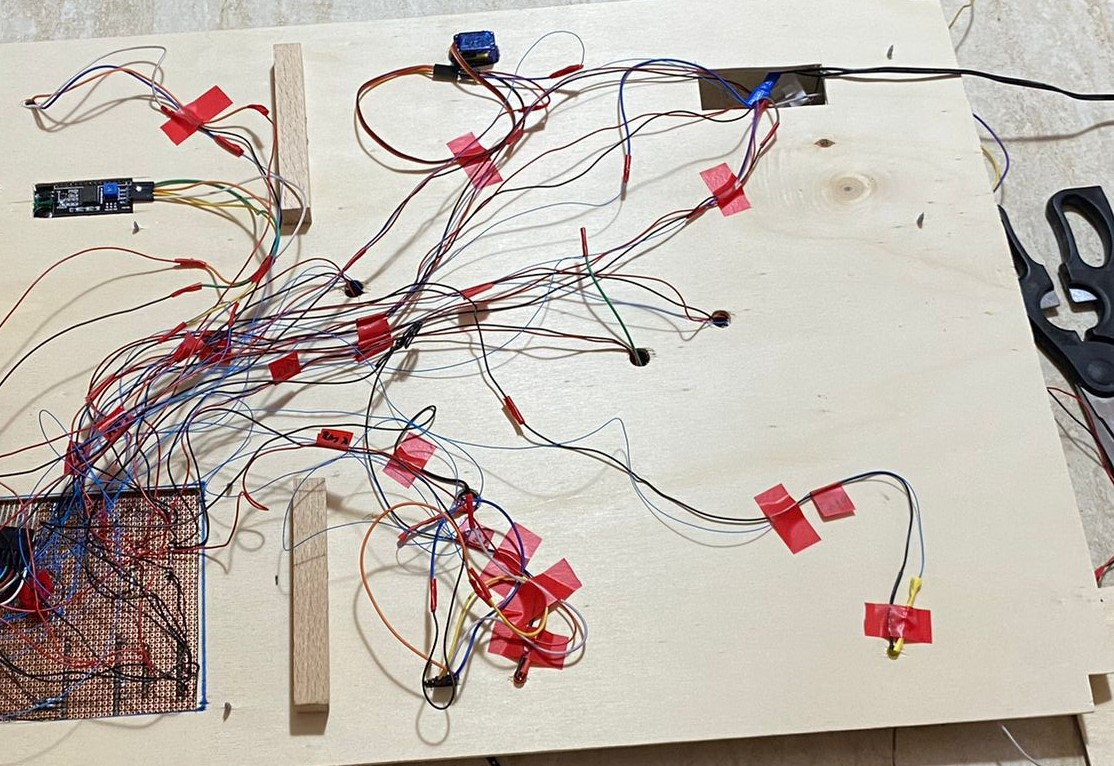
\includegraphics[width=0.6\textwidth, height=0.4\textwidth]{bachelors_ro/images/podea_dubla.jpg}
\caption{Spatele podelei duble }
\label{fig:podea_dubla}
\end{figure}

\section{Interfețe finale pentru platforma Blynk și aplicația Android}

În Figura \ref{fig:interfata_android} este prezentată interfața finală a aplicației mobile Android dedicată sistemului. Se poate observa butonul de conectare la modulul de Bluetooth și câmpul de date unde sunt afișați parametrii oferiți de senzori.

\begin{figure}[H]
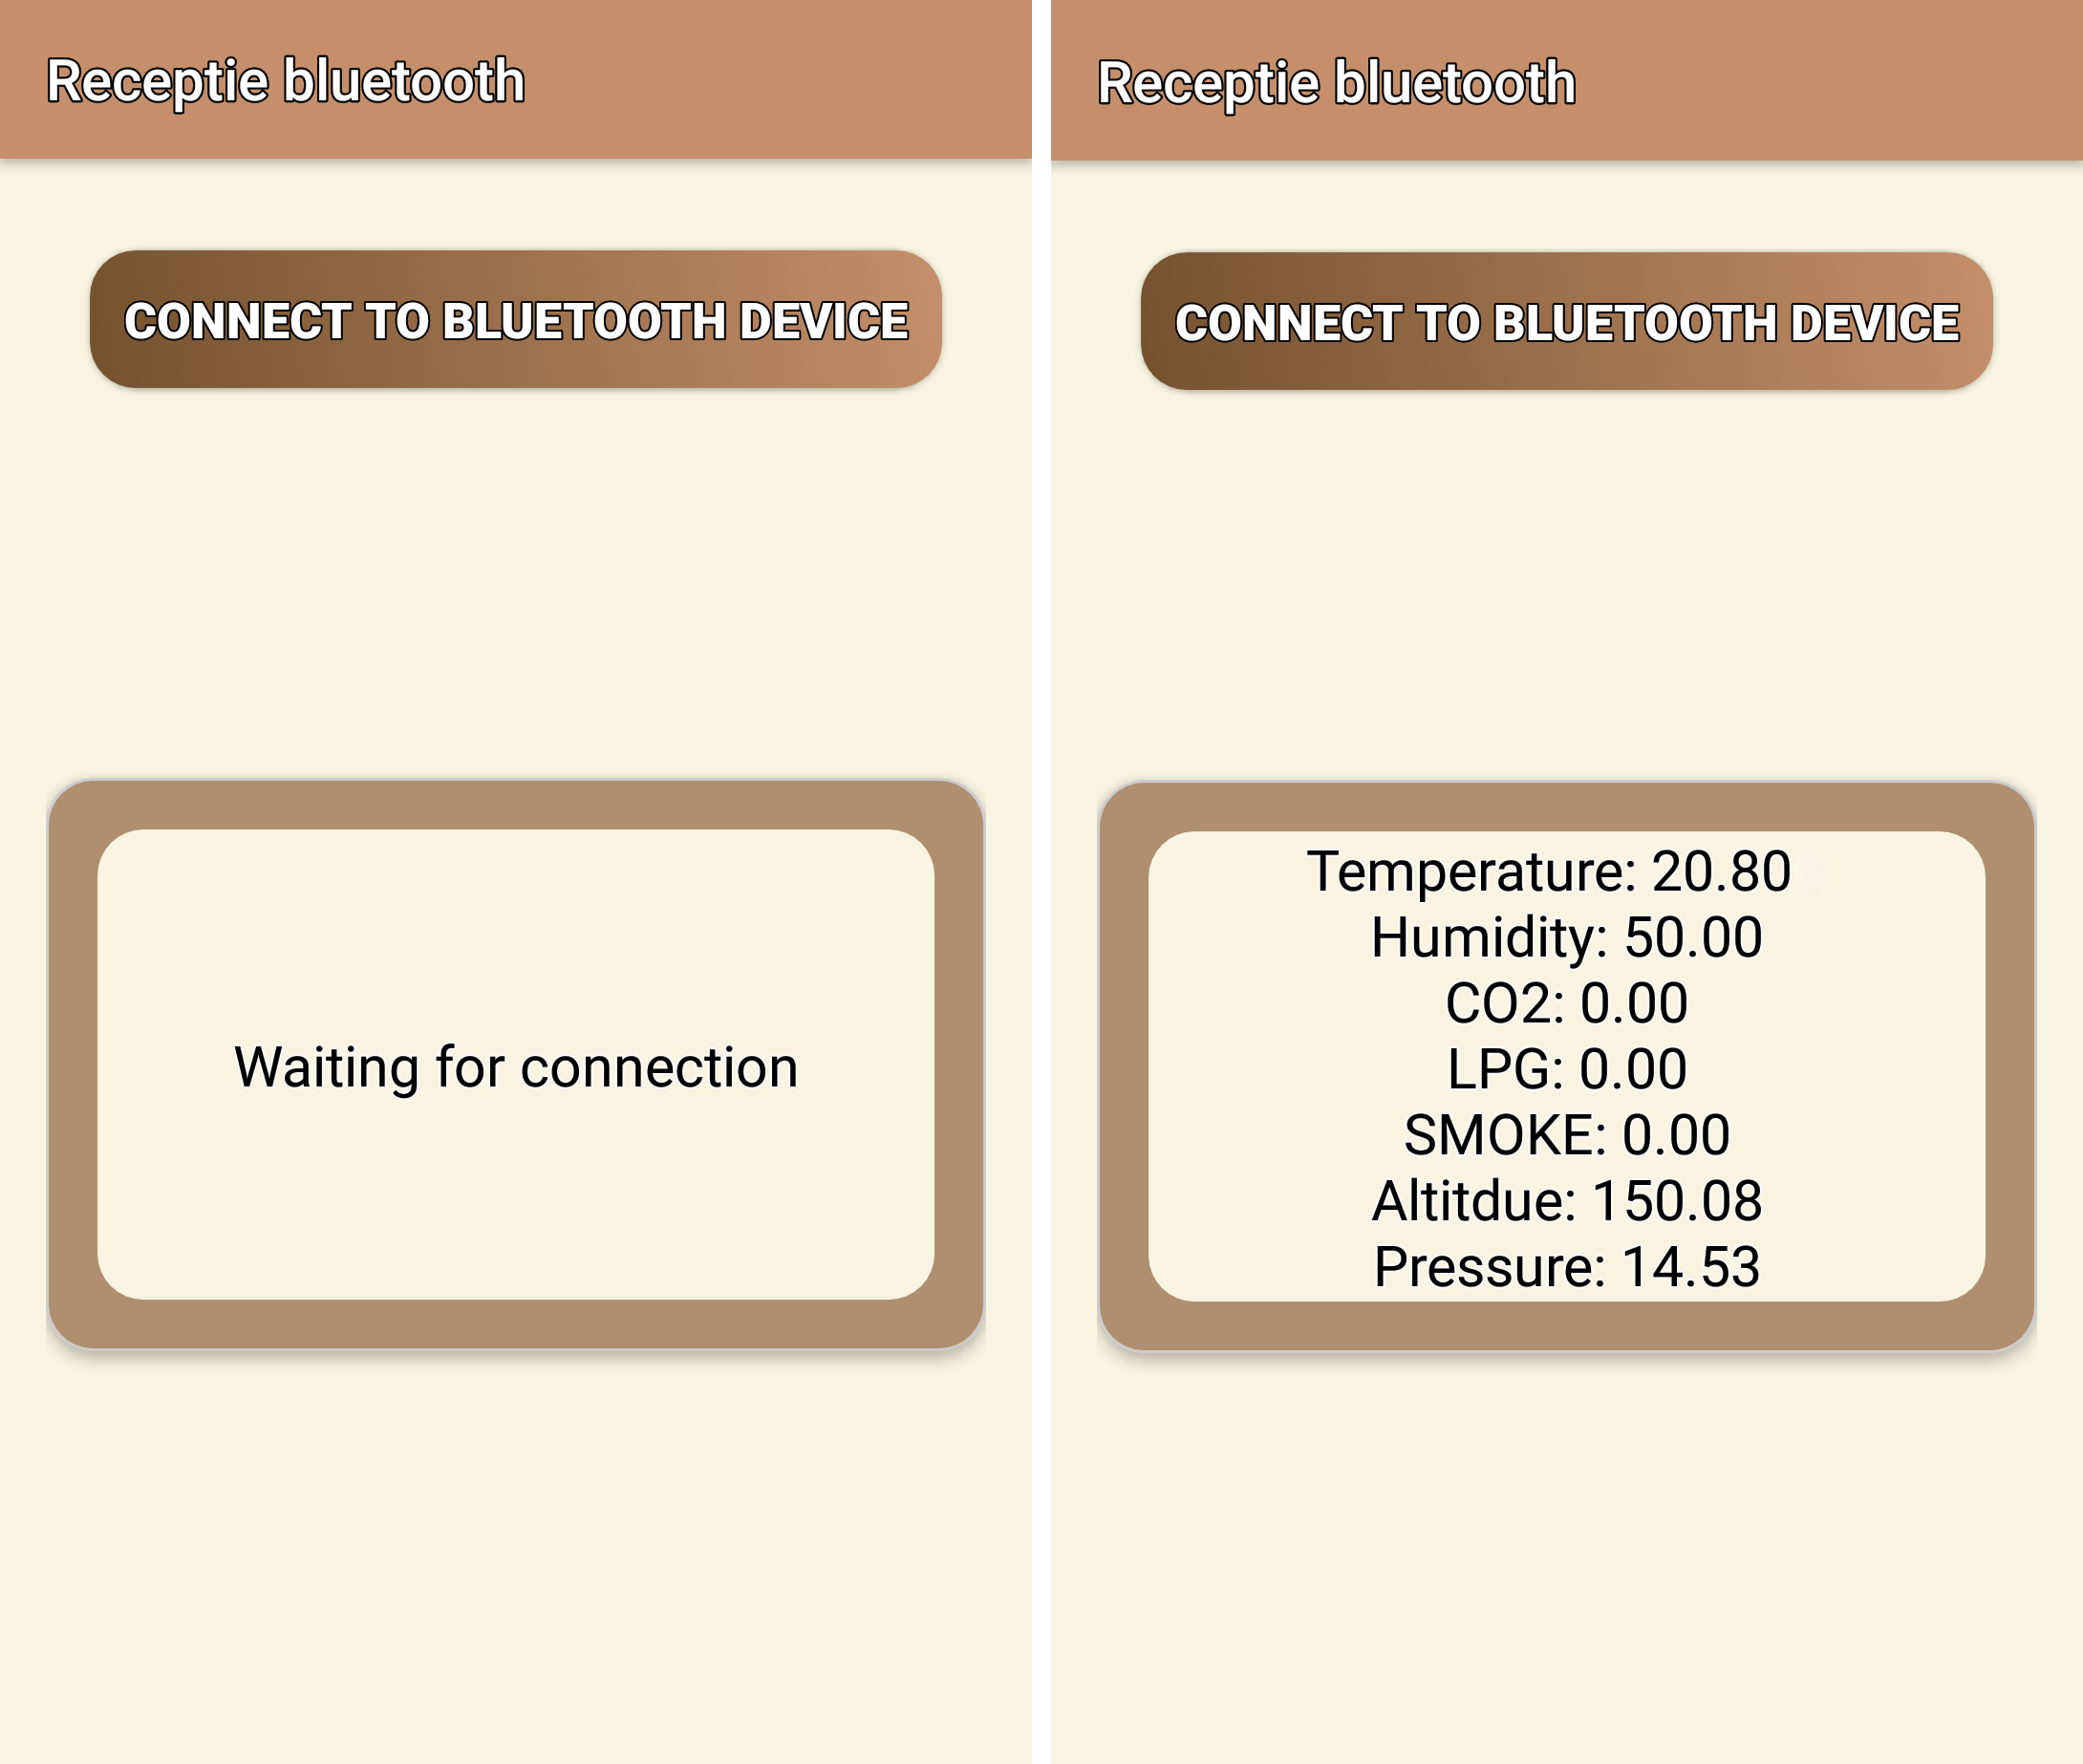
\includegraphics[width=0.6\linewidth]{bachelors_ro/images/bt_app_combined_separted.png}
\caption{Interfața aplicației mobile}
\label{fig:interfata_android}
\end{figure}

Interfețele finale web și mobile, pentru platforma Blynk, sunt prezentate în Figurile \ref{fig:interfata_blynk_web}, respectiv \ref{fig:interfata_blynk_mobile_full}.

\begin{figure}[H]
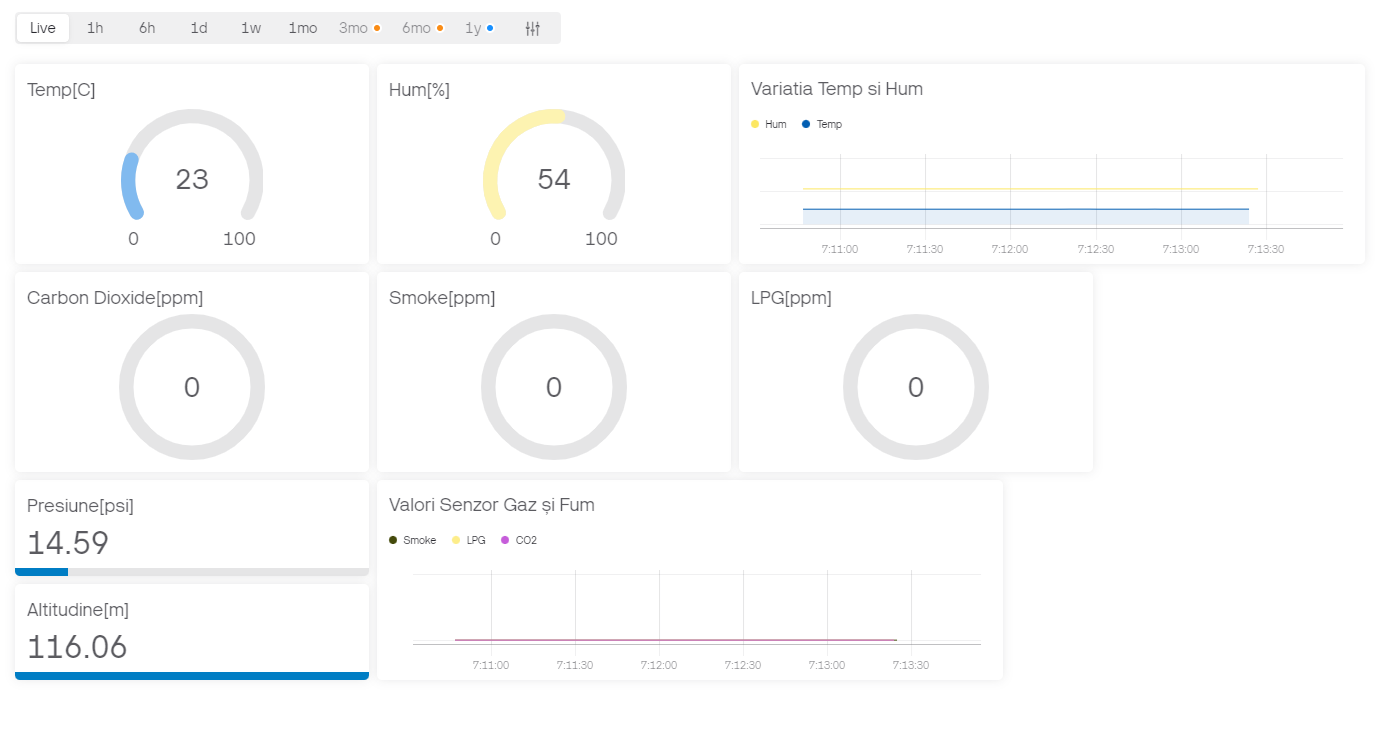
\includegraphics[width=1\linewidth]{bachelors_ro/images/interfata_blynk_web.png}
\caption{Interfața web a platformei Blynk}
\label{fig:interfata_blynk_web}
\end{figure}

\begin{figure}[H]
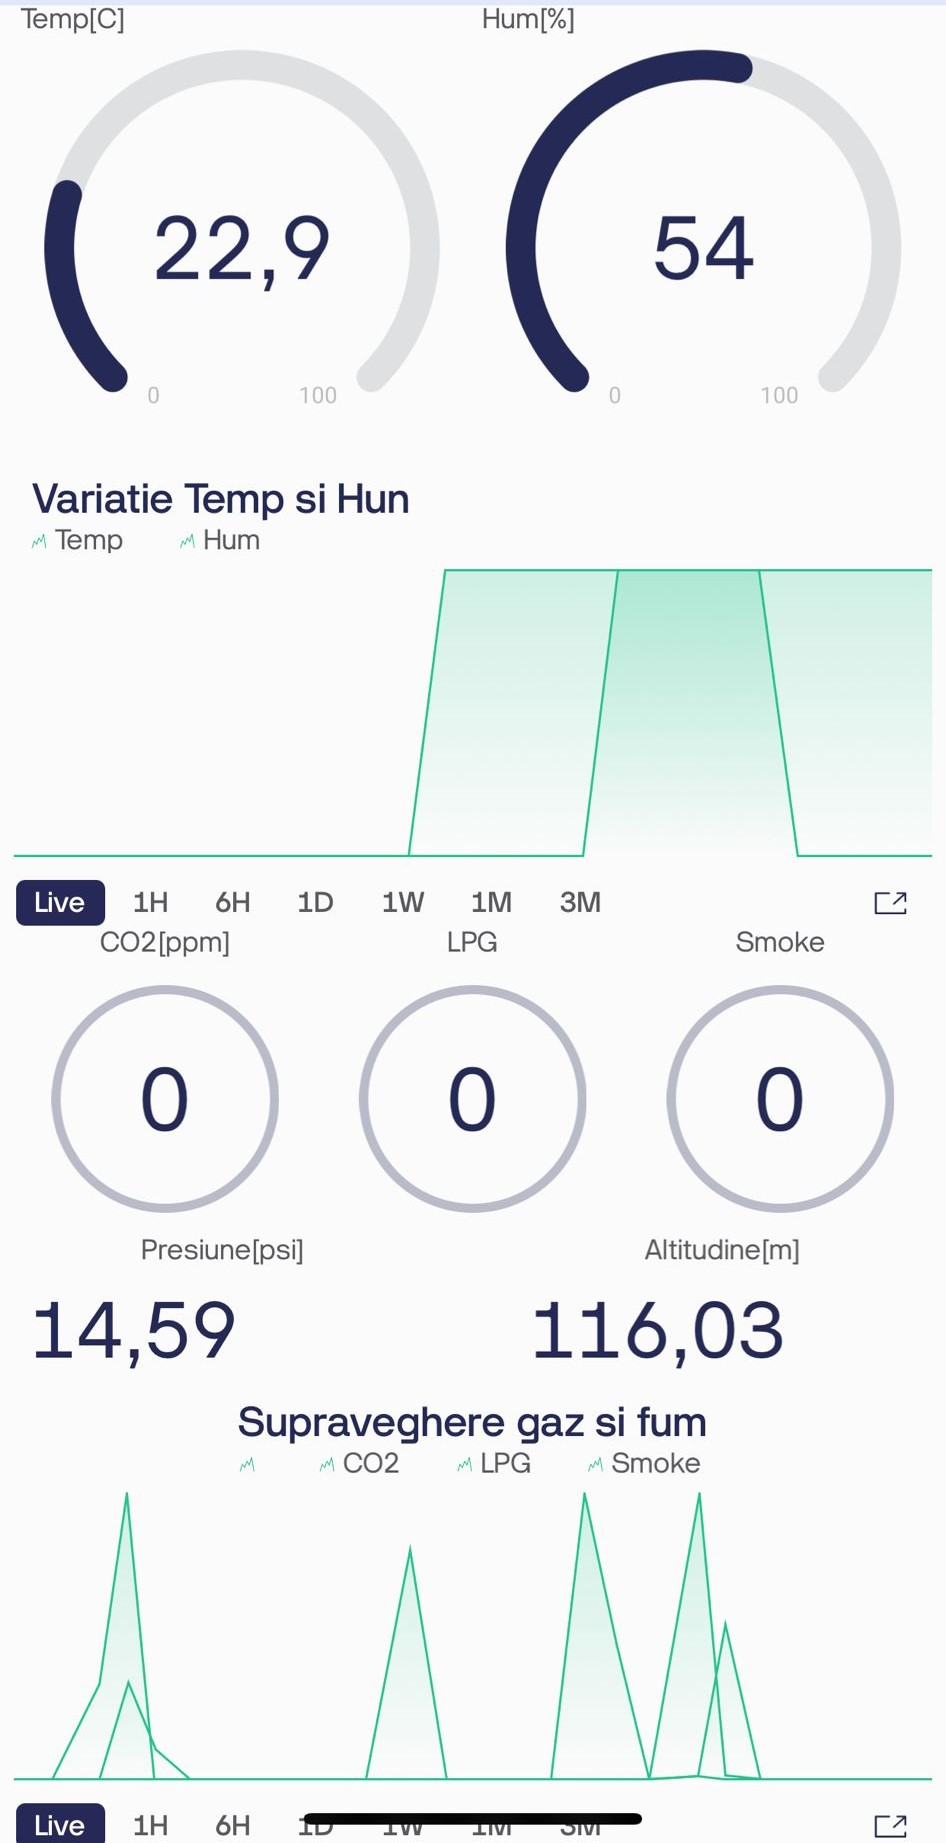
\includegraphics[width=0.3\linewidth]{bachelors_ro/images/interfata_blynk_mobile_full.jpg}
\caption{Interfața mobile a platformei Blynk}
\label{fig:interfata_blynk_mobile_full}
\end{figure}

\section{Probleme întâmpinate}

Inițial, pentru proiectul pe care urma să îl implementez, am decis să folosesc Arduino Uno, dar pe măsură ce avansam cu implementarea componentelor am realizat că placa nu oferă performanțele și tehnologiile de care aveam nevoie. Arduino Uno oferă doar un cuplu de pini pentru comunicarea serială, iar eu aveam nevoie de două. Pentru această problemă am decis să folosesc o bibliotecă de comunicare serială software\cite{software_serial_lib}, dar în scurt timp în urma experimentelor am aflat că aceasta este incompatibilă cu biblioteca necesară folosirii servomotorului\cite{servo_lib}. Acest conflict apare în urma faptului că, atât biblioteca dedicată servomotorului, cât și cea pentru comunicarea serială software împart un ceas intern de lucru oferit de placă.

Un alt impediment întâmpinat a fost numărul redus de pini digitali oferit de Arduino Uno. Această placă oferă doar 14 pini digitali din care majoritatea aveau și funcții suplimentare de care aveam nevoie cum ar fi: cei 6 pini ce dispun de PWM(Pulse Width Modulation), cei 2 pini de comunicare serială (RX, TX), cei 2 pini de comunicare prin intermediul protocolului I2C (SDA, SCL)\cite{uno_pinout}.

Ultima problemă de care m-am lovit a fost faptul că memoria flash de 32 KB oferită de Arduino Uno era aproape utilizată în întregime. Memoria SRAM de 2KB era foarte solicitată în timpul execuției programului, astfel reducea performanțele programului\cite{uno_specs}.